\documentclass[a5paper,12pt]{article}
\usepackage{../../style}


\newcommand{\montitre}{Algo Avancée }


\begin{document}

\fiche{Introduction}
\titre{Qu'est-ce qu'un problème ?} C'est une question paramétrée dans un ensemble infini. \\

\titre{Instance :} Une instance d'un problème est obtenue en spécifiant la valeur du paramètre.\\

\titre{Résolution :} Un algorithme résoud un problème s'il trouve la solution à toutes ses instances.\\ 

\titre{Heuristique :} Ressemble à un algorithme mais ne trouve pas toujours la même solution. \\

\titre{Encodage d'une instance :} On représente les instances d'un problème par une suite de symboles répondant à un schéma d'encodage.\\

\titre{Taille d'une instance :} Nombre de symboles utilisés pour la représenter.\\

\titre{Remarque :} En général, on ne s'intéresse pas au schéma d'encodage précisément mais à un critère proportionnel à la longueur d'un schéma d'encodage raisonnable.\\

\titre{Complexité temporelle d'un algorithme :} \\$f\ffonc{n}{}$ nb\_max d'étapes élémentaires pour résoudre une instance de taille $n$


\fiche{Ordres de grandeur}
\titre{$O$ :} Une fonction $f(n)$ est dans $O(g(n))$ si il existe deux constantes strictement positives $K$ et $C$ telles que 
$\forall n > k, f(n) \leq g(n)$ \\
Version équivalente : $\displaystyle{\lim_{n\rightarrow \infty} \frac{f(n)}{g(n)} < \infty}$\\

\titre{$\Omega$ :} $f(n) \in \Omega(g(n))$ si $g(n) \in O(f(n))$. \\

\titre{$\theta$ :} $f(n) \in \theta(g(n))$ si $g(n) \in O(f(n))$ et $f(n) \in O(g(n))$ \\

\titre{Propriétés du $O$ :} Soit $f$ et $g$ tq $f(n) \in O(g(n))$. Soient $a,b,c$ des constantes et $x$ une variable.
\begin{enumerate}
	\item Si $a\geq0$ et $\forall n \geq a, f(n) < g(n)$ alors $f(n) \in O(g(n))$
	\item Si $a\geq0$ alors $af(n) \in O(f(n))$
	\item Si $a\geq1$ et $b\geq0$ alors $a^{n+b}\in O(a^n)$
	\item Si $f(n)\in O(g(n))$ et $f_1(n) \in O(g_1(n))$ alors $f(n) + f_1(n) \in O(\max(g(n),g_1(n)))$
	\item Si $f(n) \in O(g(n))$ et $f_1(n) \in O(g_1(n))$ alors $f(n)f_1(n) \in O(g(n)g_1(n))$
	\item Si $a \geq 2, b \geq 1, c > 0$ alors $\log_a(n^b) \in O(n^c)$
	\item Si $a > 0$ et $b > 1$ alors $n^a\in O(b^n)$
\end{enumerate}
\newpage
\titre{preuves}
\begin{enumerate}
	\item On pose $k=a$ et $C=1$.
	\item On pose $k=1$ et $C=a$.
	\item $a^{n+b}=a^ba^n$, on applique le cas 2 avec $f(n) = a^n$
	\item On prend $(k,C)$ pour $f(n) \in O(g(n))$, $(k_1,C_1)$ pour $f_1(n) \in O(g_1(n))$ \\
			On prend $(k_2,C_2)$ avec $k_2=max(k,k_2)$ et $C_2=2\max(C,C_1)$\\ On pose $h(n) = \max(g(n),g_1(n))$ \\
			On a pour $n>k_2$ : $f(n) + f_1(n) \leq Cg(n) + C_1g_1(n) \leq \max(C,C_1)h(n) + \max(C,C_1)h(n) \leq C_2h(n)$ 
	\item On prend $(k,C)$ pour $f(n) \in O(g(n))$, $(k_1,C_1)$ pour $f_1(n) \in O(g_1(n))$ 
			On prend $(k_2,C_2)$ avec $k_2=max(k,k_2)$ et $C_2=CC_1$\\ On pose $h(n) = g(n)g_1(n))$ \\
			On a pour $n>k_2$ : $f(n)f_1(n) \leq Cg(n)C_1g_1(n) \leq \C_2h(n)$ 
	\item $\log_a(n^b) = b\log_a(n)$ donc il reste à montrer que $\log_a(n) \in O(n^c)$ \\
		Il suffit de faire $\lim \frac{\ln n}{n^c}$, qui vaut 0 par le lemme de l'hôpital.
	\item Il suffit de faire $\lim \frac{n^a}{b^n}$ avec le lemme de l'hôpital.
\end{enumerate}

\titre{Idée :} On cherche à exprimer la complexité d'un algo en fonction de la taille $n$ de l'instance en entrée. \\





\fiche{Diviser pour régner}
\titre{3 étapes :}
\begin{enumerate}
	\item Diviser le problème initial en plusieurs sous problèmes.
	\item Régner : Si la taille d'un sous problème est assez petite, on le résoud. Sinon récursion.
	\item Combiner : On forme la solution au problème initial en combinant les solutions aux sous problèmes.
\end{enumerate}

\titre{Schéma : }\\
Fonction DPR(Probleme P)\\
Debut\\
	\hspace*{1cm} Si taille(P) petite alors Resoudre(P)\\
	\hspace*{1cm} Sinon \\
		\hspace*{2cm} Diviser P en P$_1$, P$_2$, \ldots, P$_k$ \\
		\hspace*{2cm} Pour i de 1 à $k$ S$_i$ = DPR(P$_i$) FinPour \\
		\hspace*{2cm} Combiner(S$_1$,\ldots,S$_n$)\\
Fin\\

\titre{Théorème Maître:} 
\begin{itemize}
	\item Si $f(n) = O(n^{\mathrm{log}_ba-\varepsilon})$ ($\varepsilon > 0)$ alors $T(n)\in O(n^{\mathrm{log}_ba})$
	\item Si $f(n) = \theta(n^{\mathrm{log}_ba})$ alors $T(n) = O(n^{\mathrm{log}_ba}\ln n)$
	\item Si $f(n) = \Omega(n^{\mathrm{log}_ba+\varepsilon})$ ($\varepsilon > 0$). Alors $T(n) \in O(f(n))$
\end{itemize}

\newpage

\titre{Représentation des appels récursifs par un arbre :}\\

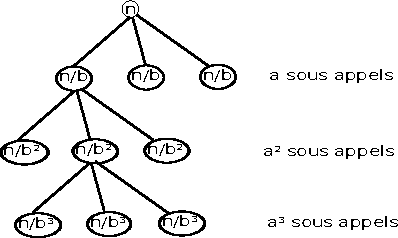
\includegraphics[width=250px]{Images/03_arbreDR.pdf}\\

\begin{tabular}{l|l|l|}
Niveau & Nb Noeuds & Temps pour ce niveau \\ \hline
0 & 1 & $f(n)$ \\ \hline
1 & $a$ & $af(\frac{n}{b})$ \\ \hline
2 & $a^2$ & $a^2f(\frac{n}{b^2})$ \\ \hline
3 & $a^3$ & $a^3f(\frac{n}{b^3})$ \\ \hline
\vdots & \vdots & \vdots 
\end{tabular}
\\
\begin{enumerate}
	\item hauteur de l'arbre : $\frac{n}{b^h} = 1 \equiv h = \log_bn$
	\item Nb de noeuds dans l'arbre : $a^0+a^1+a^2+\ldots+a^h = \frac{1+a^{h+1}}{1-a} = C + C2a^h$. Or $a^h = a^{\log_bn}=(b^{\log_ba})^{\log_bn} =  (b^{\log_bn})^{\log_ba} = n^{\log_ba}$. Donc le nombre de noeuds dans l'arbre est en $O(n^{\log_ba})$.
	\item La complexité de l'algorithme dépend ce qui compte le plus de $f(n)$ ou du nombre de noeuds dans l'arbre. Il y a donc trois cas.
\end{enumerate}





\fiche{Prog. dynamique}
\titre{Sous structure optimale :} Une solution à une instance contient en elle la solution de plusieurs sous problèmes. \\

\titre{Mémoriser } les solutions aux sous problèmes pour pouvoir les réutiliser dans le calcul de la solution. \\

\titre{Cas d'utilisation :} La programmation dynamique est souvent utile lorsqu'on a une équation de la forme $T(n) \geq aT(n-b) + f(n)$ \\

\titre{Théorème :} Soit $T(n)$ une fonction de complexité temporelle qui satisfait l'équation : \\ $T(n) = aT(n-b) + f(n)$, avec $a\geq 2, b\geq 1, f(n) \in \Omega(1)$. \\ Alors $\exist c > 1 \tq T(n) \in \Omega(c^n)$\\

\titre{Preuve :} On pose $c = \displaystyle{^b\sqrt{a}}$. Montrons par récurrence que $T(n) \geq c^n-a$. \\
Initialisation : Si $n\leq b$ alors : $c^n - a = c^n - c^b \geq 0$ (car $c>1$ et $b \geq n$). Or $T$ est une fonction de complexité donc $T(n)\geq 0$ \\
Hérédité : Si $n>b$, on suppose que $T(n-b) \geq c^{n-b}-a$. \\
On a alors $T(n) = aT(n-b) + f(n) \geq a(c^{n-b} - a) + f(n) = c^n - a^2 + f(n) \geq c^n - a^2$ (car $f(n) \geq 0$) donc $T(n) \in \Omega(c^n)$\\
\newpage
\titre{Exemple : Nombres de Fibonacci} \\
$\mathrm{Fibo}(n) = \left\{ \begin{array}{ll} 0 \; \mathrm{si} \; n=0 \\ 2 \; \mathrm{si} \; n=2 \\ f(n-1)+f(n-2) \; \mathrm{sinon} \\ \end{array} \right.$\\

\titre{Algo : Découpe de barres} \\ On dispose d'une barre de longueur $n$, et d'un tableau prix indicé de $1$ à $k$. On cherche la manière de découper la barre de façon à maximiser le prix de vente (somme des prix des sous barres). \\

\titre{Algo : Distance de Levenstein} \\
On se dote de 3 opérations sur les mots : 
\begin{enumerate}
	\item Enlever une lettre
	\item Ajouter une lettre
	\item Remplacer une lettre par une autre
\end{enumerate}
Etant donnés deux mots $u$ et $v$ on cherche le nombre minimum d'opérations élémentaires pour transformer $u$ en $v$. \\

\titre{Algo : Impression équilibrée d'un texte} \\
On veut imprimer $n$ mots sur maximum $n$ lignes de taille $N$. Les espaces donnent des pénalités. \\


\fiche{Back-Track}
\titre{Principe :} Un algo qui progresse vers une solution en faisant des choix plus ou moins arbitraires et qui revient en arrière lorsqu'il est bloqué avant d'atteindre une solution. Si tous les choix ont été explorés, on en conclut qu'il n'existe pas de solution. \\

\titre{Avantages :}
\begin{enumerate} 
	\item Facilement adaptable à beaucoup de problèmes 
	\item Facile à implémenter grâce à la récursivité
\end{enumerate}

\titre{Inconvénient :} 
\begin{enumerate} 
	\item Produit souvent une complexité exponentielle
\end{enumerate}

\titre{Algo : Sudoku} \\

\titre{Algo : Dancing Links}


\fiche{NP-complétude}
\titre{Algo polynomial :} Complexité en $O(n^k)$

\titre{Types de problèmes :}
\begin{enumerate}
	\item D : Décision (OUI ou NON)
	\item O : Optimisation (+ grande ou + petite valeur qui satisfait un critère)
	\item E : Existence (on cherche un élément qui satisfait un critère)
\end{enumerate}
La plupart des problèmes peuvent se décliner sous ces 3 formes, et si D est polynomial alors les autres aussi. On se contentera donc d'étudier la version D des problèmes. \\

\titre{Réduction polynomial :} Soient $P_1$ et $P_2$ deux problèmes.\\
On appelle réduction polynomiale de $P_1$ vers $P_2$ un algo $R$ polynomial qui transforme toute instance $I_1$ de $P_1$ en une instance $I_2$ de $P_2$ telle que $P_1(I_1) = P_2(I_2)$. \\
S'il existe une réduction polynomiale de $P_1$ vers $P_2$, on note $P_1 \leq_p P_2$. \\

\titre{Théorème :} Soient $P_1$ et $P_2$ deux problèmes tels que $P_1 \leq_p P_2$.
\begin{itemize}
	\item Si $P_2$ est polynomial alors $P_1$ aussi
	\item Si $P_1$ n'est pas polynomial alors $P_2$ non plus (forme contraposée)
\end{itemize}

\titre{Preuve} Il suffit de poser $A_1 = A_2 \circ R$. Si $A_2$ est en $O(n^k)$ et $R$ en $O(n^l)$, alors $A_1$ est en $O(n^{lk})$. \\

\titre{Equivalence polynomiale :} On dit que $P_1$ et $P_2$ sont polynomialement équivalents si $P_1 \leq_p P_2$ et $P_2 \leq_p P_1$. On le note $P_1 =_p P_2$\\

\titre{Relations :} $=_p$ est une relation d'équivalence et $\leq_p$ est une relation d'ordre. \\

\titre{Théorème :} Tous les problèmes polynomiaux sont polynomialement équivalents (même classe d'équivalence). \\

\titre{Preuve :} Soit $I_{OUI}$ et $I_{NON}$ deux instances de $P_2$ telles que $P_2(I_{OUI}) = OUI$ et $P_2(I_{NON}) = NON$. \\
Il suffit de définir ainsi l'algo $R$ : \\Si $P_1(I) = OUI$ Alors retourner $I_{OUI}$ \\ Sinon retourner $I_{NON}$

\titre{2 Classes d'équivalence utiles :} (il existe une infinité de classes d'équivalence)
\begin{itemize}
	\item P : Ensemble des problèmes pour lesquels il existe un algo qui calcule une solution en temps polynomial
	\item NP : Ensemble des problèmes pour lesquels il existe un algo de vérification en temps polynomial
\end{itemize}

\titre{NP-Difficulté} Un problème $P_0$ est NP-Difficile si pour tout problème $P_1 \in $ NP, on a $P_1 \leq_p P_0$ \\

\titre{NP-Complétude} Un problème $P_0$ est NP-Complet si : 
\begin{itemize}
	\item $P_0 \in $ NP
	\item $P_0$ est NP-Difficile
\end{itemize}

\titre{Premier problème NP-Difficile} Théorème de Cook
\begin{itemize}
	\item SAT est dans NP (le vérificateur est facile)
	\item SAT est NP-Difficile : Tout problème de NP peut être réduit en SAT :
	\begin{itemize}
		\item On part d'une instance $I$ d'un problème de NP, $V$ le vérificateur fixe, $C$ le certificate quelconque (valeur quelconque dans chaque partie de la RAM contenant $C$).
		\item On écrit une expression booléenne qui vérifie l'exécution de $V$ dans la RAM avec $I$ donné, $C$ quelconque et réponse OUI à la fin. Cette expression booléenne se construit en temps polynomial car elle est de taille polynomiale.
	\end{itemize}
\end{itemize}

\titre{SAT $\impl$ FNC $\impl$ 3-SAT} : Voir petite astuce sur le wiki pour transformer une clause en 3-clause.


\fiche{Graphes}
\titre{Clique :} Une clique de taille $n$ est un sous graphe complet de taille $n$ ($K_n$). Une anticlique de taille $n$ est un sous graphe vide de taille $n$ ($\bar{K_n}$). \\

\titre{Théorème de Ramsey :} Pour tout entier $k \geq 1, \exists R_k \in \N$ tel que tout graphe possédant au moins $R_k$ sommets contient au moins une clique ($K_k$) ou une anticlique ($\bar{K_k}$) de taille $k$. \\

\titre{Exemple :}\\
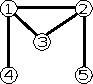
\includegraphics[width=60px]{Images/01_exRamsey.pdf} \\
$\begin{array}{|c|c|}
	 k & R_k \\ \hline
	 1 & 1 \\ \hline
	 2 & 2 \\ \hline
	 3 & 6 \\ \hline
	 4 & 18 \\ \hline
	 5 & \in [43;49] \\ \hline
	 6 & \in [102;165] \\ \hline
	 17 & \in [8917;601080389] \\ \hline
\end{array}$
\\

\titre{Essai d'algorithme naïf :} On cherche tous les graphes de chaque taille et on cherche un contre exemple. \\
Pour une taille $N$ donné il existe $2^{\frac{N(N-1)}{2}}$ graphes possibles. \\
Pour chaque graphe possible on va tester tous les sous graphes de taille $k$ donc $\frac{N!}{k!(N-k)!}$. \\
Puis pour chacun il faut vérifier que c'est une clique ou une anticlique donc $\frac{k(k-1)}{2}$. \\
Et il faut itérer sur $N$ pour chercher un contre exemple. \\
Pour $N = 8$ et $k = 4$ le programme ne terminera pas de notre vivant. \\

\titre{Représentation d'une instance :} Graphe dont les sommets sont des entiers. \\
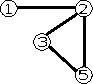
\includegraphics[width=50px]{Images/02_exEncodage.pdf}\\
Symboles = $\{ (,),0,1,2,3,4,5,6,7,8,9,- \}$. \\
Schéma = $(1-2-3-5)(1-2-3-5-2-3-2-5)$ représente le graphe ci-dessus avec une taille 26.\\

\titre{Cycle Eulérien :} Passe une et une seule fois par chacune des arêtes. \\

\titre{Théorème :} Un graphe $G$ est eulérien \ssi il est connexe et tous ses sommets sont de degré pair. \\

\titre{Preuve :}
\begin{itemize}
	\item $\impl$ Si $G$ a un sommet de degré impaire, il ne peut pas être eulérien car chaque passage dans un sommet diminue son degré de 2.
	\item $\implinv$ Si $G$ a tous ses sommets de degré pair, dès qu'on arrive sur un sommet, on peut sortir, donc on revient forcément au début. Pour chaque sommet dont tous les voisins n'ont pas été visités, on choisit une arête sortante non visitée, par le même raisonnement on revient à ce sommet au bout d'un moment. On intègre le cycle obtenu au cycle de départ et on recommence, jusqu'à ce que toutes les arêtes aient été visitées.
\end{itemize}

\titre{Cycle Hamiltonnien :} Passe une et une seule fois par chacun des sommets. \\


\fiche{Bilan problèmes}
\titre{Clique :} Existe-t-il une clique de taille $k$ dans $G$ ?\\

\titre{Ensembles indépendants :} Existe-t-il dans $G$ un ensemble de $k$ sommets sans arête commune ?\\

\titre{Couverture des arêtes :} Existe-t-il dans $G$ un ensemble de $k$ sommets tel que toute arête soit adjacente à un sommet de cet ensemble ? \\

\titre{Cycle Hamiltonnien :} Existe-t-il un cycle qui passe une et une seule fois par chaque arête. \\

\titre{Problème du voyageur de commerce :} Existe-t-il un chemin de taille $\leq k$ passant par tous les sommets ? \\

\titre{Sudoku de taille $N$ :} Grille de $N^2$ lignes, $N^2$ colonnes, $N^2$ blocs de taille $N^2$. Complétez la grille avec des nombres de $1$ à $N^2$. \\

\titre{Couverture exacte :} Etant donnée une matrice binaire $M$ sélectionner $k$ lignes de manière à avoir une et une seule occurence de 1 sur chaque colonne. \\
Solution X de type BackTrack : Pour une colonne donnée, supprimer les lignes contenant 1 sauf une, puis si X(M) alors vrai, sinon annuler la suppression et recommencer. \\

\titre{SAT, 3SAT, CSAT :} Trouver une affectation pour une conjonction de clauses. \\
 
\titre{Indé $\leq_p$ Clique :} Graphe complémentaire \\

\titre{Clique $\leq_p$ Indé :} Graphe complémentaire \\

\titre{CA $\leq_p$ Indé :} $k \rightarrow n-k$ \\

\titre{Indé $\leq_p$ Couv :} $k \rightarrow n-k$ \\

\titre{Cycle Hamiltonnien $\leq_p$ Voyageur :} Arête $\rightarrow$ poids 1 ; PasArête $\rightarrow$ poids 2 ; $k = $ nb sommets. \\

\titre{Sudoku $\leq_p$ CE :} $M$ matrice de $N^6$ lignes et $4N^4$ colonnes \\
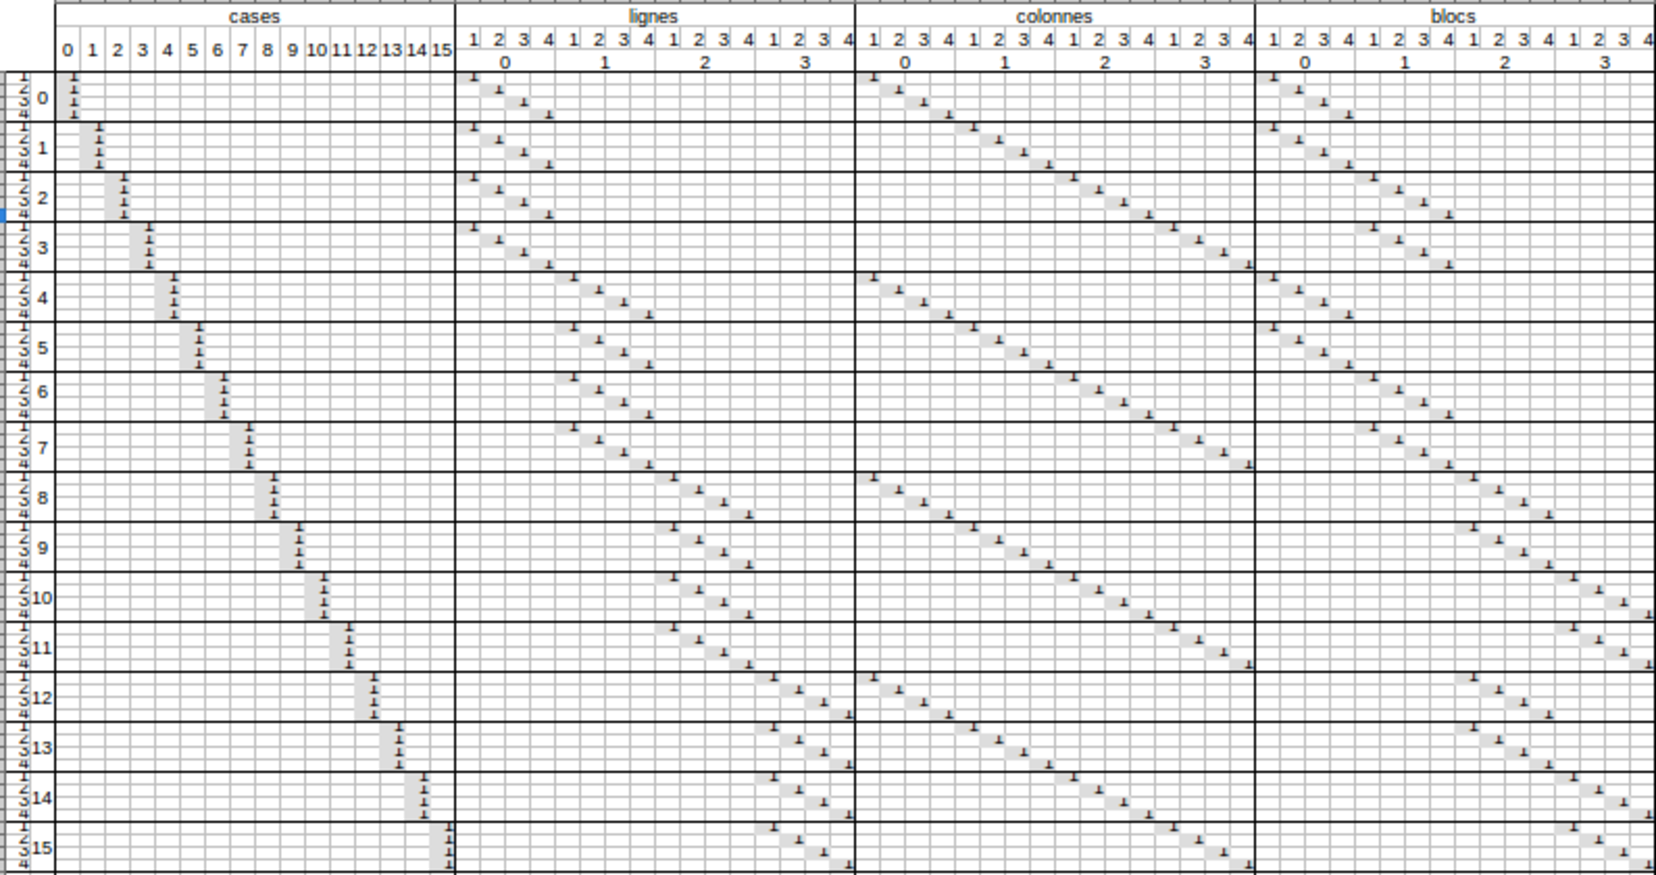
\includegraphics[width=350px]{Images/04_sudoku_couv.pdf}






\end{document}
